\documentclass[a4paper]{article}

\usepackage[pages=all, color=black, position={current page.south}, placement=bottom, scale=1, opacity=1, vshift=5mm]{background}
\SetBgContents{
	\tt Adam Zawieruhca
}      

\usepackage[margin=1in]{geometry} % full-width

% AMS Packages
\usepackage{amsmath}
\usepackage{amsthm}
\usepackage{amssymb}

% Unicode
\usepackage[utf8]{inputenc}
\usepackage{hyperref}
\hypersetup{
	unicode,
%	colorlinks,
%	breaklinks,
%	urlcolor=cyan, 
%	linkcolor=blue, 
	pdfauthor={Author One, Author Two, Author Three},
	pdftitle={A simple article template},
	pdfsubject={A simple article template},
	pdfkeywords={article, template, simple},
	pdfproducer={LaTeX},
	pdfcreator={pdflatex}
}

% Vietnamese
%\usepackage{vntex}

% Natbib
\usepackage[sort&compress,numbers,square]{natbib}
\bibliographystyle{mplainnat}

% Theorem, Lemma, etc
\theoremstyle{plain}
\newtheorem{theorem}{Theorem}
\newtheorem{corollary}[theorem]{Corollary}
\newtheorem{lemma}[theorem]{Lemma}
\newtheorem{claim}{Claim}[theorem]
\newtheorem{axiom}[theorem]{Axiom}
\newtheorem{conjecture}[theorem]{Conjecture}
\newtheorem{fact}[theorem]{Fact}
\newtheorem{hypothesis}[theorem]{Hypothesis}
\newtheorem{assumption}[theorem]{Assumption}
\newtheorem{proposition}[theorem]{Proposition}
\newtheorem{criterion}[theorem]{Criterion}
\theoremstyle{definition}
\newtheorem{definition}[theorem]{Definition}
\newtheorem{example}[theorem]{Example}
\newtheorem{remark}[theorem]{Remark}
\newtheorem{problem}[theorem]{Problem}
\newtheorem{principle}[theorem]{Principle}

\usepackage{graphicx, color}
\graphicspath{{fig/}}

%\usepackage[linesnumbered,ruled,vlined,commentsnumbered]{algorithm2e} % use algorithm2e for typesetting algorithms
\usepackage{algorithm, algpseudocode} % use algorithm and algorithmicx for typesetting algorithms
\usepackage{mathrsfs} % for \mathscr command

\usepackage{lipsum}

% Author info
\title{Hierarchical Bloom Filters: A Page Fault Reducing Bloom Filter
\author{Adam Zawierucha (adz2)}

\date{
	Rice University \\ zawie@rice.edu}%
%	\today
}


\begin{document}
	\maketitle
	
	\begin{abstract}
		Bloom filters \cite{Bloom} are used ubiquitously due to their speed and memory efficiency in theory and in practice.
        However, the default implementation of sufficiently large bloom filters sets and reads bits appearing in different physical pages of memory,
        which results in an increase in page faults. In general, increase memory usage increases page faults which in turn slows down programs \cite{TAY200699}. 
        In this paper we propose a bloom filter implementation that guarantees one page access per insert or query, minimizing page faults.
        The implementation we propose implements the abstract bloom filter operations on a collection of baby bloom filters with a size equal to the system's page size.
        We will show theoretically and empirically that this implementation is expected to be faster than the default implementation.

		\noindent\textbf{Keywords:} probabilistic data structures, bloom filters, memory hierarchy, implementation, page fault analysis
	\end{abstract}
	

	\section{Descripton}
	In this section I will describe the proposed hierarchial blooom filter implementaiton in detail.

	Our hierarchial bloom filter will be a collection of bloom filters of the computer systems page size (4096 bytes).
	We will have as many bloom filters as it takes to occupy $M$ bits. $M$ sohuld be $10N$ where $N$ is the number of expected keys to be in the bloom filter.
	We will generate $8$ independent hash functions. 1 hash function will be used to select the sub-bloom filter; the other $7$ will be used to set bits in the baby bloom filter as the standard implementation.

	The idea behind this is that we minimize page faults, as we only need to access one page of memory to set bits instead of up to $7$.

	The numbers selected will be justified in the \textit{Theoretical Justification} section.
	
	\section{Literature Survey}
	In my literature survey, I discovered a similar approach except making bloom filters hierarchial.
	Tim Kaler's proposed cache-efficient bloom filters \cite{Kaler} makes sub-bloom filters of size cache-size; thus, their idea is very similar to mine except they do it on a smaller unit of memory.

	Evgeni Krimer and Mattan Erez used a power-of-two choice principle within blocked-bloom filters to decrease the false positive rate.
	Instead of simply selecting one block to write into, they choose multiple.
	\cite{Krimer}.

	\section{Performance Theoretical Justification}
	Asymptotically, we expect no difference between the variantions.
	However, real life computer systems have memory hierarchy;
	in essence, certain parts of memory are faster to access than others.
	One unit of memory is a PAGE -- typically a 4096 contiguous block of physical memory.
	The standard variation sets bits accross a virtually contiguous block of $M$ bits of memory.
	However, physically this is subdivided into pages. 
	Thus, for sufficiently large $M$ it becomes increasingly likely that the bits set and read by the standard implementation will origin from distinct physical pages.
	In fact, for a bloom filter of size $100$ pages and $k=7$, we expect to hit $6.8$ pages. Thus, we can make up to $7$ page faults.
	
	
	\begin{proof}
		Let $M$ denote the number of bits in the bloom filter. 
		Let $P$ denote the number of bits in a page. 
		Let $k$ denote the number of hash functions used.

		Let $A$ be a random variable denoting the number of pages accessed.
		Let $A_i$ be an indicator variable indicting whether or not page $i$ is accessed.
		$$E(A_i) = P(\text{page $i$ is not accessed by any of the $k$ hash functions})$$
		$$E(A_i) = 1 - (P(\text{a hash function does not access page $i$}))^k$$
		$$E(A_i) = 1 - (1-P(\text{a hash function hits page $i$}))^k$$
		$$E(A_i) = 1 - (1-\frac{1}{M/P})^k$$
		$$E(A_i) = 1 - (1-\frac{P}{M})^k$$

		By the linearity of expectation:
		
		$$E(A) = \Sigma_0^{M/P} (1 - (1-\frac{P}{M})^k)$$
		$$E(A) = \frac{M}{P}(1 - (1-\frac{P}{M})^k)$$
		When we set $k=7$, $\frac{M}{P} = 100$ (in other words, we use 100 pages of memory), we see that:

		$$E(A) = 6.8$$

		% We will now apply Markov's inequality.
		% $$P(A \geq a) = \frac{E(X)}{a} = \frac{M}{Pa}(1 - (1-\frac{P}{M})^k)$$

		% When we set $k=7$, $\frac{M}{P} = 100$ (in other words, we use 100 pages of memory), and $a = 7$ (all hash functions are set)
		% We see that:

		% $$P(A \geq 7) = P(A = 7) \leq 97\%$$
	\end{proof}

	
	
	
	
	Thus, the standard implementation expects to see in the vincity of $k$ page faults for sufficiently large $M$. 
	
	Our hierarchial bloom filter gaurentees $1$ page fault. This is trivially true as we contructed a hash function which decided which page we will write all our bits into. Thus, our implementation will experience as many or less page faults!
	Thus, we expect higher throughput as the operating systems does not have to load and store pages of memory as frequently.


	\section{False Positive Theoeretical Justification}
	In this section, we will justify theoretically why our implementaiton will have a similar false positive rate.

	\subsection{Standard}
	The anticipated false postive rate of the standard implementation of bloom filter is:
	\begin{equation}
		f_p = (1-(1-\frac{1}{m})^{nk})^k
	\end{equation}
	\subsection{Hierarchical}
	\begin{equation}
		f_p = (1-(1-\frac{1}{m})^{nkl})^{kl}
	\end{equation}
	Where $l$ is the number of sub-bloom filters to access. And $k$ is the number of hash functions to use per sub-bloom filter.

	For similar reasons, the optimal value for $kl = 7$. Thus, we select $l=1$ and $k=7$ to minimize page access while minimizing the false positive rate.
	This assumes $m = 10n$.
	\section{Experiments}

	I run three experiments on my data structure.

	\subsection{Measure False Positive Rate}
	
	For this experiment, we seek to measure how the false positive rate of our Hierarchical bloom filter compares to the standard bloom filter. 
	Our theoeritcal anaylsis shows that these should be equivalent.
	
	\textbf{Hypothesis:} \textit{The hierarchial bloom filter will have an identical false positive rate.}

	\subsubsection{Experimental Settings}
	The experiment will run as follows. First, generate $N$ random keys to insert and $N$ random keys to query by that are all distinct from the insertion keys.
	We choose $N= 2,000,000$. Then, for each bloom filter variant, generate bloom filters of various sizes: a bloom filter with $2N$ bits, $3N$ bits, $\ldots$ to $15N$ bits. 
	Generate the bloom filter with the parameters that theoertically minimize false positive rate; i.e $k=7$, $l=1$.
	Then, for each sized bloom filter, insert our $N$ keys for insertion and query $N$ false keys and compute what precentage of them are falsely accepted.
	This measurement is the false positive rate of the variant for a certain bits per element measurement.
	Repeat this experiment $20$ times and take the average. (The plots I generated in results only do it once, for now.)
	This gives us a good gauge of how false positive rate behaves for each variant as we provide more memory.
	
	Ideally, we want to see the Hierarchical bloom filter having the same false positive rate as the standard bloom filter.

	\subsubsection{Results}
	\begin{center}
		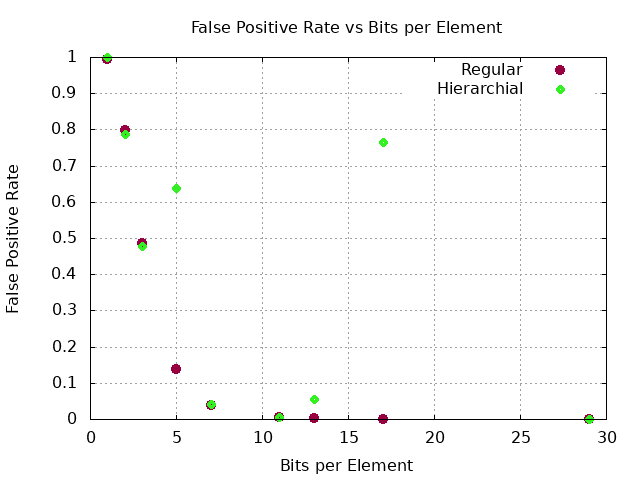
\includegraphics[width=10cm]{../plots/fp.png}
	\end{center}

	We can see interesting results here. 
	The hierarchial bloom filter has substantially worse false positive rates sometimes. 
	You can see sometimes the false positive bad becomes extraordinarily bad. 
	These upticks are likely due to bad selections of seed for the choke-point hash function. Thus, this leads to a lot of collisions and therefore a high false positive rate.

	For the filnal paper I will run the experiment multiple times and mean to get a more meaningful result.

	Nonetheless, this demonstrates a flaw in my proposed data structure which I will discuss more in my final paper.
	It is interesting that the theoeretical analysis predicts that they will have the same bound, but in practice we see worse false positive rate.
	\subsection{Measure Throughput for small $m$}
	
	For this experiment, we seek to validate two things 
	\begin{enumerate}
		\item The run time is constant with respect to the size of the bloom filter
		\item The hierarchical bloom filter has similar speeds to the standard bloom filter for low page sizes.
	\end{enumerate}

	\textbf{Hypothesis:} \textit{The hierarchial bloom filter will work the same 1 page size, and slowly become better but platue when the page count becomes 7.}
	\subsubsection{Experimental Settings}
	The experiment will run as follows.
	First, generate $N=10,000,000$ random keys. 

	Then, we will run the following experiment on the two variants and plot the results.
	Use the optimal theoeretical configuraiton for each bloom filter (i.e, $k=7$, $l=1$)
 	\begin{enumerate}
		\item Generate a bloom filter of size $m$ pages.
		\item Insert all $N$ keys and time how long it takes to do the operation; we will denote the elapsed time as $t$
		\item Compute and plot the throughput: $N/t$
	\end{enumerate}
	Repeat the experiment for $m = 1,2,\ldots,8,9,10,15,20,25$

	\subsubsection{Results}
	\begin{center}
		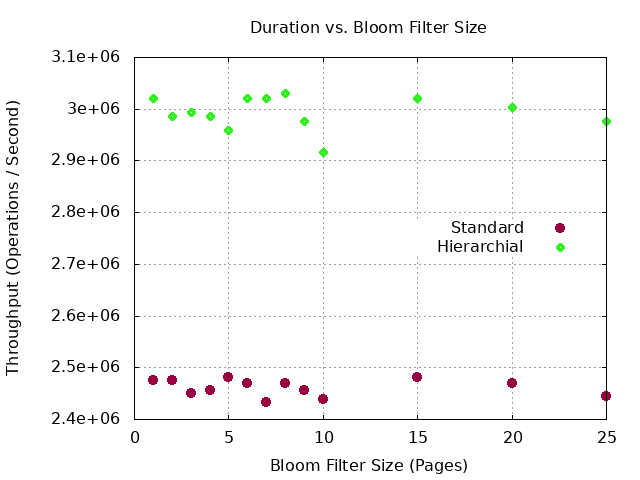
\includegraphics[width=10cm]{../plots/scale-m.png}
	\end{center}

	These results are positive: the hierarchial bloom filter has higher throughput than the standard bloom filter.

	However, I have unexplained results as my bloom filter should behave identically when $m=1$. This will be explored for the final paper.
	It is possible I miss computed or made a coding error in one or both of the implementations. This requires more digging...
	\subsection{Measure Duration as $n$ scales}

	For this experiment, we seek to validate that our implementation performs better than the standard implementation as $n$ grows.
	
	\textbf{Hypothesis:} \textit{The hierarchial bloom filter will take less time to insert $n$ keys}

	\subsubsection{Experimental Settings}
	
	The experiment will run as follows:
 	\begin{enumerate}
		\item Generate $n = 500,000$ keys
		\item Generate a bloom filter of both varianets of size $10n$. Use the optimal theoeretical configuraiton for each bloom filter (i.e, $k=7$, $l=1$).
		\item Time how long it takes to insert all $n$ keys into each of the bloom filters.
		\item Plot the time and results.
		\item Repeat for $n = 1e6, 2e6, \ldots 120e6$
	\end{enumerate}

	\subsubsection{Results}
	\begin{center}
		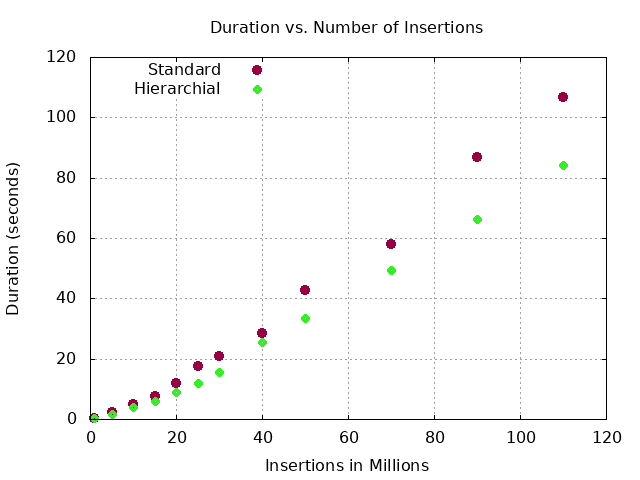
\includegraphics[width=10cm]{../plots/scale-nm.png}
	\end{center}

	These results are positive: the hierarchial bloom filter takes noticably less time to insert $n$ keys for every choice of $n$.
	I will do more numerical analysis for the final paper. But these results are promising!
	\newpage
	\bibliography{refs}

	
\end{document}